\documentclass[landscape]{tikzposter}
%%%<
\usepackage{verbatim}
%%%>
\begin{comment}
:Title: Poster with TikZ
:Tags: Mathematics;Graphics;TikZ;Classes;Geometry;Functions;Plots;Chapter1
:Author: Stefan Kottwitz
:Slug: poster

We know for example informational or scientific posters seen at conferences or at walls in universities or institutes.

They mostly have certain characteristics in common:

- They have a large size, such as A2, A1 or even A0.

- People may look at them from far away, but also from a very close distance.

In consequence, we got some requirements for typesetting:

- Page layout dimensions should work with such a big size.

- We need a wide range of font sizes. We should be able to read while standing close, but we also need large catchy headings.

- The poster should be partitioned into digestible blocks. Specifically, each block should not exceed the usual line width we know from body texts. Also here applies, that too wide lines would make it hard to focus and to skip back to the start of the next line. So, lines in blocks should not be much wider than about 40 or 50 characters long.

- Blocks should have distinct headings.

- Graphical elements such as colors and lines can be used to divide in parts.

- Images should be vector graphics or should have a high resolution.

Here, we would like to create a poster of A0 size in landscape orientation.
It shall show some blocks containing dummy text as place holder, math,
and images. As sample images, we will take fractals which I made for
http://texample.net, and a plot and a geometry drawing from Chapter 10,
Advanced Mathematics.
In the book, we included the images as files. Here, we create them
completely within the poster document, to have a single self-contained document.
You can later replace the dummy text and other parts by your own content.

We will use the tikzposter class. The document is structured
in columns and blocks. 

The code is fully explained in the LaTeX Cookbook, Chapter 1,
The Variety of Document Classes, Creating a poster.
\end{comment}
\usetheme{Wave}
\usepackage{pgfplots}% for the 3D plot
\usepackage{tkz-euclide}% for geometry
\usetkzobj{all}
\usepackage{lipsum}% for dummy text
\usepackage{multicol}% for multiple columns
\usetikzlibrary{lindenmayersystems,shadings}% gives us fractals
\pgfdeclarelindenmayersystem{Koch curve}{
  \rule{F -> F-F++F-F}}
\pgfdeclarelindenmayersystem{Sierpinski triangle}{
  \rule{F -> G-F-G}
  \rule{G -> F+G+F}}
\pgfdeclarelindenmayersystem{Fractal plant}{
  \rule{X -> F-[[X]+X]+F[+FX]-X}
  \rule{F -> FF}}
\pgfdeclarelindenmayersystem{Hilbert curve}{
  \rule{L -> +RF-LFL-FR+}
  \rule{R -> -LF+RFR+FL-}}
\setlength{\columnsep}{4cm}
\setlength{\columnseprule}{1mm}
\newcommand*{\image}[2][]{% For conveniently including images
  \begin{tikzfigure}[#1]
    \includegraphics[width=\linewidth]{#2}
   \end{tikzfigure}}
\usepackage{lmodern}
\renewcommand*{\familydefault}{\sfdefault}% Let's have a sans serif font
\begin{document}
\title{\LaTeX\ in Use}
\author{John Doe}
\maketitle
\begin{columns}
  \column{.65}
  \block{Fractals in \LaTeX}{
    \lipsum[1]
    %\image[\LaTeX\ workflow]{flowchart}% if external
    \tikz\shadedraw[shading=color wheel,scale=2] 
      [l-system={Koch curve, step=2pt, angle=60, axiom=F++F++F, order=4}]
        lindenmayer system -- cycle;\hfill
    \tikz\shadedraw [top color=white, bottom color=blue!80,scale=3,
      draw=blue!80!black] [l-system={Sierpinski triangle, step=2pt,
      angle=60, axiom=F, order=7}] lindenmayer system -- cycle;\hfill
    \tikz\shadedraw [bottom color=white, top color=red!80,scale=3,
      draw=red!80!black][l-system={Hilbert curve, axiom=L, order=4,
      step=8pt, angle=90}] lindenmayer system; \hfill
    \tikz\draw [green!50!black, rotate=90,scale=2]
      [l-system={Fractal plant, axiom=X, order=5, step=2pt, angle=25}]
      lindenmayer system;\hfill
    \tikz\shade[shading=Mandelbrot set] (0,0) rectangle (15,15);
  }
  \begin{subcolumns}
    \subcolumn{.5}
    \block{Mathematics}{
      Take a coffee, then:
      \vspace{1.4cm}
      \coloredbox{\begin{itemize}
        \item State
        \item Proof
        \item Write in \LaTeX
      \end{itemize}}
      \vspace{1.4cm}
      \innerblock{Integral approximation}{
        \[
          \int_a^b f(x) dx \approx (b-a)
            \sum_{i=0}^n w_i f(x_i)
        \]
      }
    }
    \note[targetoffsetx = 4.5cm, targetoffsety = -5cm,
      angle = -30, connection, width=10cm]{\Large Weight function}
    \subcolumn{.5}
    \block{Geometry}{
    \vspace{-3cm}
    \centering
    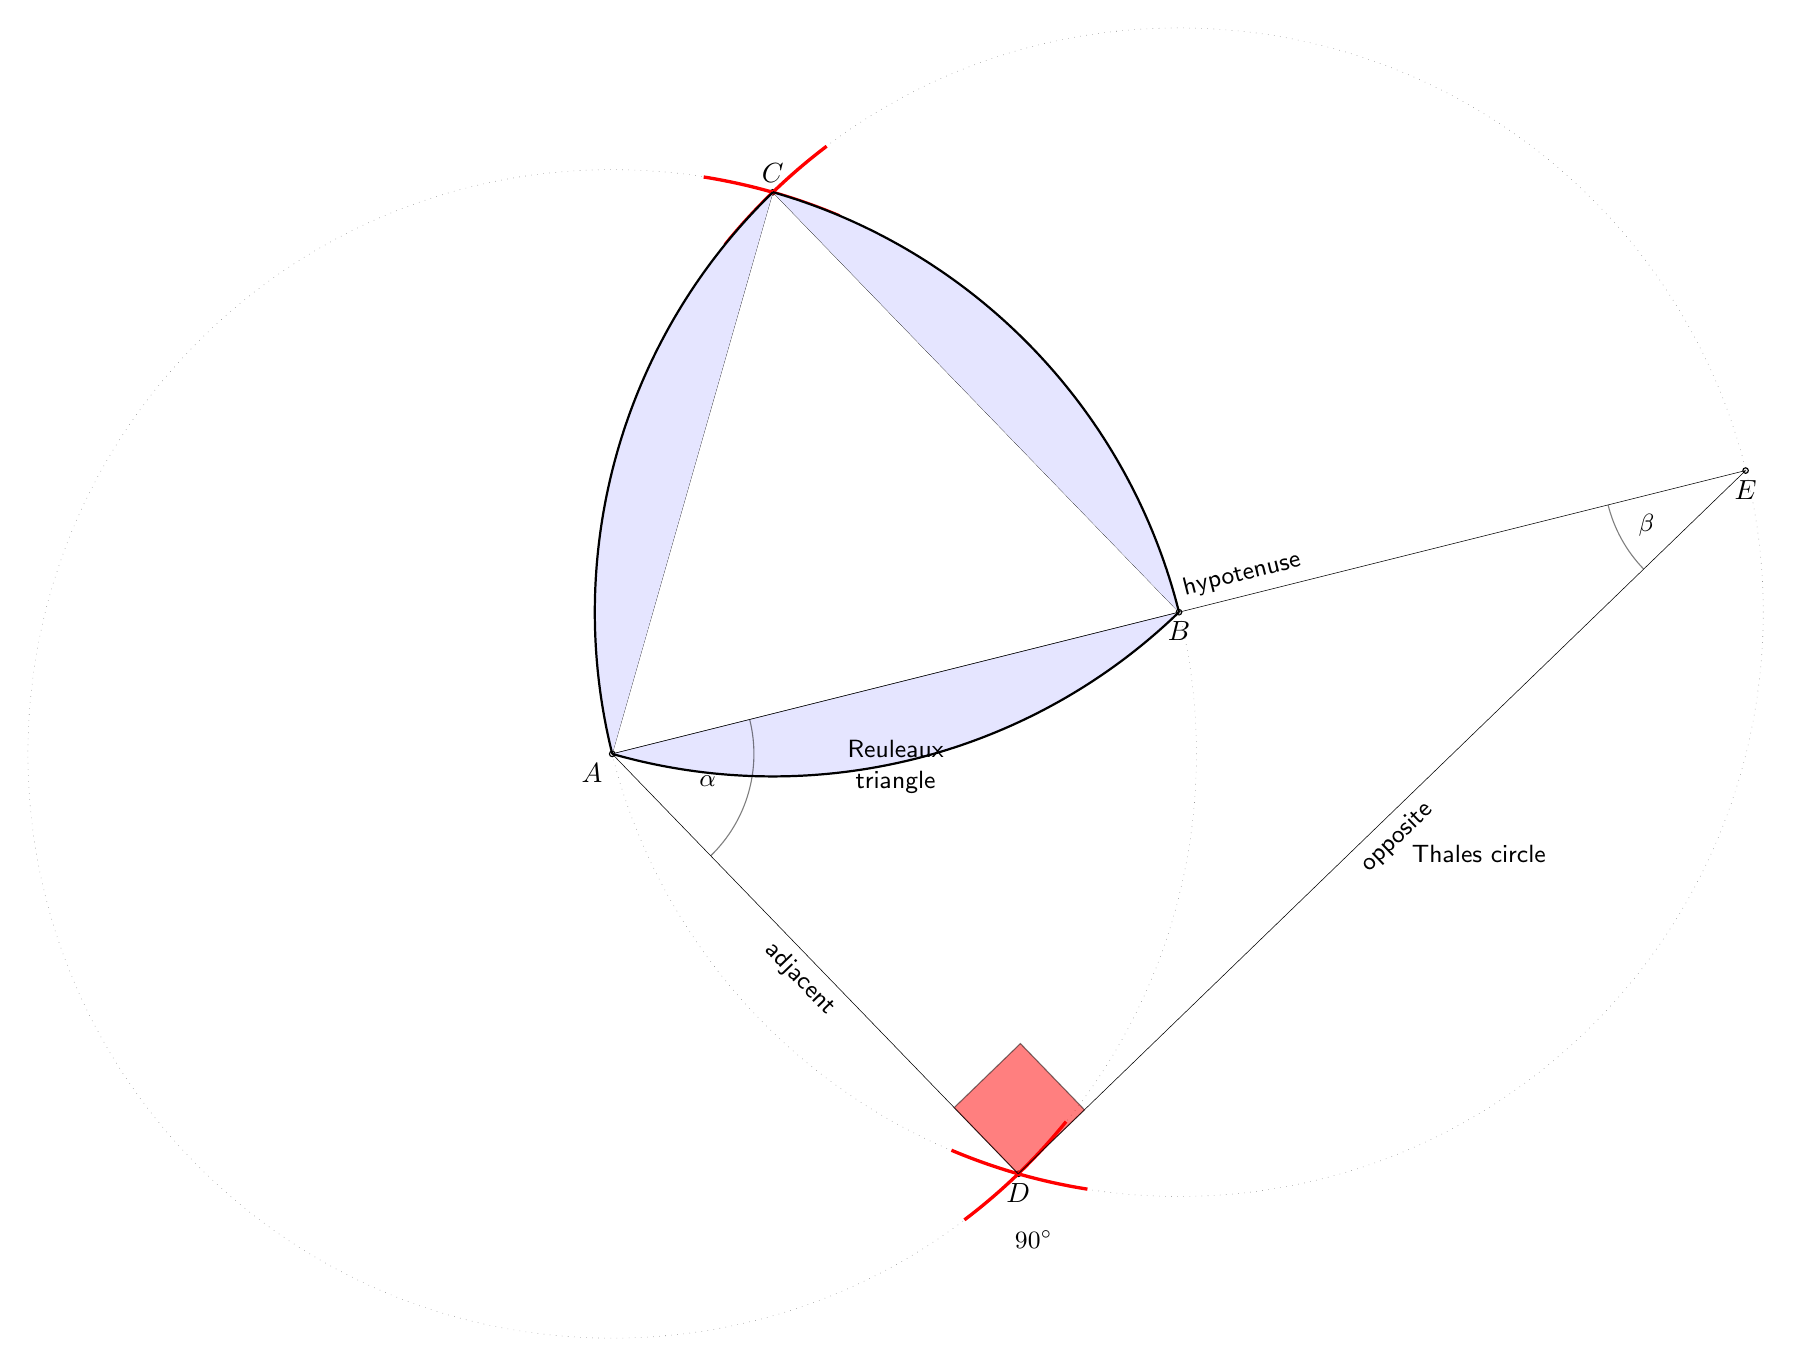
\begin{tikzpicture}[scale=1.8]
      \tkzDefPoint(0,0){A}
      \tkzDefPoint(4,1){B}
      \tkzInterCC(A,B)(B,A)
      \tkzGetPoints{C}{D}
      \tkzDrawPolygon(A,B,C)
      \tkzDrawPoints(A,B,C,D)
      \tkzLabelPoints[below left](A)
      \tkzLabelPoints(B,D)
      \tkzLabelPoint[above](C){$C$}
      \tkzDrawCircle[dotted](A,B)
      \tkzDrawCircle[dotted](B,A)
      \tkzCompass[color=red, very thick](A,C)
      \tkzCompass[color=red, very thick](B,C)
      \tkzCompass[color=red, very thick](A,D)
      \tkzCompass[color=red, very thick](B,D)
      \tkzDrawArc[fill=blue!10,thick](A,B)(C)
      \tkzDrawArc[fill=blue!10,thick](B,C)(A)
      \tkzDrawArc[fill=blue!10,thick](C,A)(B)
      \tkzInterLC(A,B)(B,A)
      \tkzGetPoints{F}{E}
      \tkzDrawPoints(E)
      \tkzLabelPoints(E)
      \tkzDrawPolygon(A,E,D)
      \tkzMarkAngles[fill=yellow,opacity=0.5](D,A,E A,E,D)
      \tkzMarkRightAngle[size=0.65,fill=red,opacity=0.5](A,D,E)
      \tkzLabelAngle[pos=0.7](D,A,E){\small$\alpha$}
      \tkzLabelAngle[pos=0.8](A,E,D){\small$\beta$}
      \tkzLabelAngle[pos=0.5,xshift=-1.4mm](A,D,D){\small$90^\circ$}
      \tkzLabelSegment[below=0.6cm,align=center,font=\small](A,B){Reuleaux\\triangle}
      \tkzLabelSegment[above right,sloped,font=\small](A,E){hypotenuse}
      \tkzLabelSegment[below,sloped,font=\small](D,E){opposite}
      \tkzLabelSegment[below,sloped,font=\small](A,D){adjacent}
      \tkzLabelSegment[below right=4cm,font=\small](A,E){Thales circle}
    \end{tikzpicture}    
  }
  \end{subcolumns}
  \column{.35}
  \block{Plotting functions}{
    %\image{plot}% if you would like to include an external image
    \pgfplotsset{width=\linewidth}
    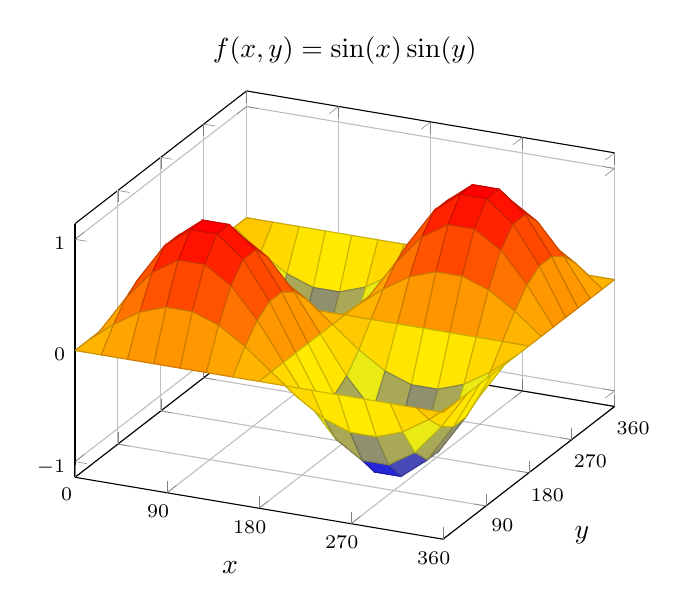
\begin{tikzpicture}
      \begin{axis} [
        title = {$f(x,y) = \sin(x)\sin(y)$},
        xtick = {0,90,...,360},
        ytick = {90,180,...,360},
        xlabel = $x$, ylabel = $y$,
        ticklabel style = {font = \scriptsize},
        grid
      ]
      \addplot3 [surf, domain=0:360, samples=15]% raise samples if desired 
        { sin(x)*sin(y) };
      \end{axis}
    \end{tikzpicture}
    \lipsum[4]
  }
\end{columns}
\block{Conclusion and outlook}{
  \begin{multicols}{4}
    \lipsum[1-2]
  \end{multicols}
}
\end{document}
